%\usepackage{xr}

% \externaldocument{note01}
% \externaldocument{note02}
% \externaldocument{note03}
% \externaldocument{note04}
% \externaldocument{note05}
% \externaldocument{note06}
% \externaldocument{note07}
% \externaldocument{note08}
% \externaldocument{note09}
% \externaldocument{note10}
% \externaldocument{note11}

\graphicspath{{./input/graphs/note01/}}

% \zexternaldocument{note01}
% \zexternaldocument{note02}
% \zexternaldocument{note03}
% \zexternaldocument{note04}
% \zexternaldocument{note05}
% \zexternaldocument{note06}
% \zexternaldocument{note07}
% \zexternaldocument{note08}
% \zexternaldocument{note09}
% \zexternaldocument{note10}
% \zexternaldocument{note11}
% \externaldocument{note12}


\week{1}
\lecture{1}{Intro and Complex Numbers}

\section{Introduction}

These notes cover the fundamental concepts of complex variables. The course begins with the basics of complex numbers, their algebra, and geometry.
We then move to sequences, series, and power series, and finally to the core concepts of analytic functions, Cauchy-Riemann equations, and various related theorems and applications.

% \section{Week 1: Lecture 1}

\subsection{Motivation}

What is the use of complex functions and complex variables? One of many things is to compute the actual value of real convergent series. 
For example, we know that the series $\sum_{n=1}^\infty \frac{1}{n^2}$ converges.
The question is, what is the value of the sum:  $\sum_{n=1}^\infty \frac{1}{n^2} = ?$
Towards the end of this module, we will be able to compute the answer. We will see:

\begin{itemize}
    \item $1 + \frac{1}{2^2} + \frac{1}{3^2} + \dots = \frac{\pi^2}{6}$
    \item $1 + \frac{1}{2^4} + \frac{1}{3^4} + \dots = \frac{\pi^4}{90}$
    \item $1 + \frac{1}{2^6} + \frac{1}{3^6} + \dots = \frac{\pi^6}{945}$
\end{itemize}

Using complex functions we will be able to compute quite complicated (real!) integrals, which may be very hard to compute otherwise, and a lot of other things. For example: Compute $\int_{-\infty}^{\infty} \frac{1}{x^4+1} dx = ?$

\section{The Field of Complex Numbers}

We start with the basic definitions, properties, and the geometry of complex numbers.

\subsection{Basic definitions and algebra}

\begin{definition}
A \emph{complex number} is an ordered pair of real numbers, $(x, y)$.  If $y = 0$, we get the pair $(x, 0) = x$ (which we denote simply by $x$).
\end{definition}

Since real numbers are a part of complex numbers, the algebraic operations (sum, subtraction, multiplication, division) on complex numbers need to be such that they agree with the corresponding algebraic operations on real numbers.  We denote $\mathbb{C}$ as the set of all complex numbers.

\begin{definition}
Two complex numbers $z_1 = (x_1, y_1)$ and $z_2 = (x_2, y_2)$, $z_1, z_2 \in \mathbb{C}$, are \emph{equal} if and only if $x_1 = x_2$ and $y_1 = y_2$.
\end{definition}

\begin{definition}
The \emph{sum} of two complex numbers $z_1 = (x_1, y_1)$ and $z_2 = (x_2, y_2)$ is a complex number $z_1 + z_2 = (x_1 + x_2, y_1 + y_2) = z_3 \in \mathbb{C}$.
\end{definition}

\begin{definition}
The \emph{product} of two complex numbers $z_1 = (x_1, y_1)$ and $z_2 = (x_2, y_2)$ is a complex number $z_1 z_2 = (x_1 x_2 - y_1 y_2, x_1 y_2 + x_2 y_1) = z_3 \in \mathbb{C}$.
\end{definition}
It is easy to see that if we apply this rule to real numbers, we get the usual product.
For $x_1,x_2 \in \mathbb{R}$: $x_1=(x_1,0)$, $x_2=(x_2,0)$
\[ (x_1,0)(x_2,0) = (x_1x_2-0 \cdot 0, x_1 \cdot 0 + 0 \cdot x_1) = (x_1x_2,0) = x_1x_2. \]
Usually, we will write a complex number as $z=x+iy$, where $i=(0,1)$.  $i$ is an ordered pair (0,1).
Let us compute $i^2$ using definition 1.4:
\[ i^2 = (0,1)(0,1) = (0 \cdot 0 - 1 \cdot 1, 0 \cdot 1+ 1\cdot 0) = (-1,0) = -1. \]
It is easy to check the usual rules for arithmetic, namely the axioms of a field.

\begin{proposition}
If $z_1, z_2, z_3 \in \mathbb{C}$, then:
\begin{enumerate}
    \item \textbf{Closure:} $z_1 + z_2 \in \mathbb{C}$, $z_1 z_2 \in \mathbb{C}$.
    \item \textbf{Commutativity:} $z_1 + z_2 = z_2 + z_1$, $z_1 z_2 = z_2 z_1$.
    \item \textbf{Associativity:} $z_1 + (z_2 + z_3) = (z_1 + z_2) + z_3$, $z_1 (z_2 z_3) = (z_1 z_2) z_3$.
    \item \textbf{Distributivity:} $z_1 (z_2 + z_3) = z_1 z_2 + z_1 z_3$.
    \item \textbf{Zero and Identity:} $z + 0 = z$, $z \cdot 1 = z$.
    \item \textbf{Negative and Inverse:} $z + (-z) = 0$, where for $z = x + iy$, $-z = -x - iy$.  If $z \neq 0$, then $z \cdot z^{-1} = 1$, where $z^{-1} = \frac{x}{x^2 + y^2} - i \frac{y}{x^2 + y^2}$.
\end{enumerate}
\end{proposition}

\begin{proof}
Let us prove the Inverse. As for the rest: (\verifythis) - check at home (all parts follow from the analogous properties of real numbers).

$z \cdot z^{-1} = (x+iy) \left( \frac{x}{x^2+y^2} - i \frac{y}{x^2+y^2} \right) = \frac{x^2 - ixy + ixy - i^2y^2}{x^2 + y^2} + i \cdot 0 = \frac{x^2+y^2}{x^2+y^2} + i \cdot 0= 1.$
\end{proof}

We will see why the inverse is defined in exactly this way.

\begin{definition}
Let $z = x + iy \in \mathbb{C}$. $x$ is called the \emph{real part} of $z$ and denoted by $x = \Re(z)$; $y$ is called the \emph{imaginary part} of $z$, denoted by $y = \Im(z)$.
\end{definition}

The algebraic form $x+iy$ to write complex numbers allows us to add and multiply complex numbers as polynomials, but remember that $i^2 = -1$.  For example:

$(x_1 + iy_1)(x_2 + iy_2) = x_1x_2 + ix_1y_2 + iy_1x_2 + i^2y_1y_2 = (x_1x_2 - y_1y_2) + i(x_1y_2 + y_1x_2)$.

% \section{Week 1: Lecture 2}
\lecture{2}{more on Complex Numbers.}

\begin{example}
 Let $z_1=1+i$, $z_2 = 2-i$. Compute $z_1+z_2$, $z_1z_2$, $z_2^{-1}$.

\begin{soln} 
$z_1+z_2 = (1+i)+(2-i)=(1+2)+(1+(-1))i = 3$
$z_1z_2 = (1+i)(2-i) = (1 \cdot 2 + i(-i)) + i (1(-1)+1\cdot 2) = 3+i$
$z_2^{-1}$: $\Re(z_2) = x=2$, $\Im(z_2) = y=-1 \implies z_2^{-1} = \frac{x}{x^2+y^2} -i \frac{y}{x^2+y^2} = \frac{2}{5} + i \frac{1}{5}$
\end{soln}
\end{example}

\subsection{Complex conjugate and division}

\begin{definition}
The \emph{complex conjugate} of the complex number $z = x + iy$ is the complex number given by $\bar{z} = x - iy$ (the bar denotes the operation of complex conjugation).
\end{definition}

\begin{remark}
\checkthis{On your own mate.}
\begin{enumerate}
    \item $\overline{(\bar{z})} = z$
    \item $\overline{z_1 + z_2} = \bar{z_1} + \bar{z_2}$
    \item $\overline{z_1 z_2} = \bar{z_1} \bar{z_2}$
    \item $\Re(z) = \frac{1}{2}(z + \bar{z}) = \frac{1}{2}(x + iy + x - iy) = x$
    \item $\Im(z) = \frac{1}{2i}(z - \bar{z}) = \frac{1}{2i}(x + iy - x + iy) = y$
\end{enumerate}
\end{remark}

Using addition and multiplication we can define subtraction and division.
\begin{definition}
Subtraction: $z_1-z_2$ is a complex number $z_3$ such that $z_1 = z_2+z_3$.
\end{definition}
Using this definition we obtain: $z_3 = (x_1-x_2) + i(y_1-y_2)$

\begin{definition}
Division: Let $z_2 \neq 0$. $\frac{z_1}{z_2}$ is a complex number $z_3$ such that $z_1 = z_2z_3$.
\end{definition}
Let us calculate $z_3$. From the definition for $z_1 = x_1+iy_1$, $z_2 = x_2+iy_2$, $z_3=x_3+iy_3$ we get:
$z_1 = x_1 + iy_1 = (x_2+iy_2)(x_3+iy_3) = (x_2x_3-y_2y_3) + i (y_2x_3+x_2y_3) = z_2z_3$
Using the equality definition we have the following system of equations:
\begin{equation*}
\begin{cases}
\Re(z_1) = x_1 = x_2x_3-y_2y_3 = \Re(z_2z_3)\\
\Im(z_1) = y_1 = y_2x_3+x_2y_3 = \Im(z_2z_3)
\end{cases}
\end{equation*}
Let us solve this system: the unknowns are $x_3$, $y_3$. Solving it gives:
\[ x_3 = \frac{x_1x_2+y_1y_2}{x_2^2+y_2^2}, \quad y_3 = \frac{x_2y_1-x_1y_2}{x_2^2+y_2^2} \]
Therefore,
\[ z_3 = \frac{z_1}{z_2} = \frac{x_1x_2+y_1y_2}{x_2^2+y_2^2} + i \frac{x_2y_1-x_1y_2}{x_2^2+y_2^2} \]

In particular, we obtain for $1/z$: $x_1=1, y_1=0, x_2=x, y_2=y$,
\[ \frac{1}{z} = \frac{1 \cdot x+ 0 \cdot y}{x^2+y^2} +i \frac{x \cdot 0 - 1 \cdot y}{x^2+y^2} = \frac{x}{x^2+y^2} -i \frac{y}{x^2+y^2} \]
Note that in the denominator we have $z_2\bar{z_2} = (x_2+iy_2)(x_2-iy_2) = x_2^2+y_2^2$.

Therefore, the recipe for division is: multiply the numerator and the denominator by the complex conjugate of the denominator and separate the real and imaginary parts.

\begin{example}
Calculate $z=\frac{3+4i}{1-i}$.

\begin{soln} 
\[ z = \frac{3+4i}{1-i} = \frac{3+4i}{1-i} \cdot \frac{1+i}{1+i} = \frac{3+3i+4i+4i^2}{1^2-(-1)^2} = \frac{-1+7i}{2} = -\frac{1}{2} + i\frac{7}{2} \]
\end{soln}
\end{example}

\begin{example}
 Prove that for any $z\in\mathbb{C}$, $\frac{z+\bar{z}}{z\bar{z}} \in \mathbb{R}$.
 
 \begin{soln}  $\frac{z+\bar{z}}{z\bar{z}} = \frac{z}{z\bar{z}} + \frac{\bar{z}}{z\bar{z}} = \frac{1}{\bar{z}} + \frac{1}{z} = \frac{z+\bar{z}}{z\bar{z}} = \frac{2\Re z}{\lvert z\rvert^2} = \frac{2x}{x^2+y^2} \in \mathbb{R}$.
 \end{soln}
\end{example}

\begin{definition}
The \emph{modulus} of $z = x + iy$ is $\lvert z\rvert = \sqrt{x^2 + y^2}$.
\end{definition}
\begin{remark}
$\lvert z\rvert \ge 0$ always and $\lvert z\rvert = 0 \iff z = 0 \iff x = y = 0$.
\end{remark}

% $\check{this}$
\checkthis{(Simple relation)} $\lvert z\rvert\ge \Re(z)$ and $\lvert z\rvert \ge \Im(z)$.
Observe: $\lvert z\rvert = \sqrt{x^2+y^2} \implies \lvert z\rvert^2 = z\bar{z} \implies \frac{1}{z} = \frac{\bar{z}}{\lvert z\rvert^2}$ if $z\neq 0$.

In the following proposition we list and prove the properties of the modulus of a complex number.
\begin{proposition}\label{proposition:1.2}
Let $z,w \in \mathbb{C}$. Then
\begin{enumerate}
    \item $\lvert zw\rvert = \lvert z\rvert  \lvert w   \rvert $
    \item $\lvert z+w\rvert \le \lvert z\rvert + \lvert w \rvert $ \hfill (Triangle Inequality)
    \item $\lvert z-w\rvert \ge\lvert \lvert z\rvert -  \lvert w   \rvert \rvert $ \hfill (Reverse Triangle inequality)
\end{enumerate}
\end{proposition}

\begin{proof}
    \begin{enumerate}
        \item Observe that (commutativity):
        $\lvert z w \rvert^2 = (zw)(\overline{zw}) = (zw)(\bar{z}\bar{w}) = (z\bar{z})(w\bar{w}) = \lvert z\rvert^2 \lvert w \rvert ^2 $ (for any $z_1,z_2$: $\overline{z_1z_2}=\bar{z_1}\bar{z_2}$).
        This proves 1) after taking square roots.
        
        \item By the definition:
        For any $z_1$, $z_2$: $\overline{z_1+z_2} = \bar{z_1}+\bar{z_2}$.
        \begin{equation*}            
            \begin{aligned}
                 \lvert z+ w \rvert^2 &= (z+w)(\bar{z}+\bar{w}) = (z+w)(\overline{z+w}) = z\bar{z} + w\bar{w} + z\bar{w} + \bar{z}w \\
                &= \lvert z\rvert^2 +  \lvert w \rvert ^2 + z\bar{w} + \overline{(z\bar{w})} = \lvert z\rvert^2+ \lvert w \rvert ^2 + 2\Re(z\bar{w}) \\                  
                & \boxed{\forall z, w : w\bar{w} = \bar{w}w, \, z\bar{z} = \bar{z}z; \quad  z+\bar{z} = 2\Re(z)} \\
                & \leq \lvert z\rvert^2+ \lvert w \rvert ^2+2 \lvert z\bar{w}\rvert = \lvert z\rvert^2+ \lvert w \rvert ^2+2\lvert z\rvert  \lvert w   \rvert = \lvert z\rvert^2+ \lvert w \rvert ^2+2\lvert z\rvert \lvert w  \rvert \\
                &= (\lvert z\rvert+ \lvert w \rvert )^2. \\
                & \boxed{(\lvert z_1z_2\rvert =\lvert z_1\rvert \lvert z_2 \rvert  \forall z_1, z_2).}
            \end{aligned}
            \end{equation*}
        \item We employ the trick of adding zero and apply 2).
        
        \begin{equation}\label{eq:trianglineq} \tag{4}
        \lvert z\rvert =\lvert (z-w)+w\rvert \leq\lvert z- w \rvert+ \lvert w  \rvert \implies \lvert z- w \rvert \geq \lvert z\rvert- \lvert w   \rvert  
    \end{equation} 
        %   (4)

        Similarly: 
        \begin{equation} \label{eq:reversetrianglineq} \tag{5}
            \lvert w-z\rvert = \lvert -(z-w)\rvert = \lvert z-w\rvert \geq  \lvert w \rvert -\lvert z\rvert 
        \end{equation}  
        
    \end{enumerate}
Combining \ref{eq:trianglineq} and \ref{eq:reversetrianglineq} we get 3).
\end{proof}
\begin{example}
Prove that if $\lvert z_1 \rvert =\lvert z_2 \rvert =1$, then $\frac{z_1+z_2}{1+z_1z_2} \in \mathbb{R}$.

\begin{soln} 
First multiply and divide by the complex conjugate of the denominator.
Denominator $1+z_1z_2 = \overline{1+z_1z_2} = 1+\bar{z_1}\bar{z_2}$
\begin{align*}
  \frac{z_1+z_2}{1+z_1z_2} &= \frac{z_1+z_2}{1+z_1z_2} \cdot \frac{1+\bar{z_1}\bar{z_2}}{1+\bar{z_1}\bar{z_2}} \\
  &= \frac{z_1+z_2+z_1\bar{z_1}\bar{z_2}+z_2\bar{z_1}\bar{z_2}}{1+z_1z_2+\bar{z_1}\bar{z_2}+z_1z_2\bar{z_1}\bar{z_2}} \\
  &= \frac{(z_1+\bar{z_1}) + (z_2+\bar{z_2})}{ \lvert 1+z_1z_2 \rvert ^2 } (\rvert z_1 \lvert=\rvert z_2 \lvert =1)\\
  &= \frac{2\Re(z_1)+2\Re(z_2)}{ \lvert 1+z_1z_2 \rvert ^2 } \in \mathbb{R}
\end{align*}
\end{soln}
\end{example}

\begin{example}
Prove that $\frac{z-1}{z+1}$ is purely imaginary iff $\lvert z\rvert=1$.

\begin{soln} (Purely imaginary, namely its real part is equal to 0)
Denominator $z+1 = \bar{z}+1$
\[ \frac{z-1}{z+1} = \frac{z-1}{z+1} \cdot \frac{\bar{z}+1}{\bar{z}+1} = \frac{z\bar{z}-z+\bar{z}-1}{ \lvert z+1 \rvert ^2 } = \frac{\lvert z\rvert^2-1 + (z-\bar{z})}{ \lvert z+1 \rvert ^2 } = \frac{\lvert z\rvert^2-1 + 2i\Im(z)}{ \lvert z+1 \rvert ^2 } \]

Note that $\lvert z\rvert^2 \in \mathbb{R}$, $\lvert z+1 \rvert ^2  \in \mathbb{R}$, $\Im(z) \in \mathbb{R}$.
\[ \Re(\frac{z-1}{z+1}) = \frac{\lvert z\rvert^2-1}{ \lvert z+1 \rvert ^2 } \quad \Im(\frac{z-1}{z+1}) = \frac{2\Im(z)}{ \lvert z+1 \rvert ^2 } \]
\[ \Re(\frac{z-1}{z+1}) = 0 \iff \frac{\lvert z\rvert^2-1}{ \lvert z+1 \rvert ^2 } = 0 \iff \lvert z\rvert^2-1 = 0 \iff \lvert z\rvert^2=1 \iff \lvert z\rvert=1 \]
\end{soln}
\end{example}

% \section{Week 2: Lectures 2+3}
\lecture{2+3}{Geometry in Complex Numbers. WO00o0W.}

\section{Geometric Representation of Complex Numbers}
% Modulus and Argument. Polar Form}

\subsection{Modulus and Argument. Polar Form}

Any complex number $z = a + ib$ can be numerically described as a point in the plane with the coordinates $(a, b)$ or as a vector that starts at the origin $(0, 0)$ and ends at the point $(a, b)$.
$iy$ $\Im z$ Imaginary axis
$ib$  Point in the plane $\mathbb{R}^2$: $(a,b)$.
$(a,b) = z = a+ib$ OR vector connecting $(0,0)$ and $(a,b)$.

% \begin{figure}
%     \centering
    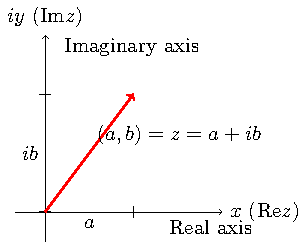
\includegraphics{complex_plane.pdf}
    % \includegraphics[width=0.8\textwidth]{figures/graph.pdf}
    % \caption{My compiled graph}
    % \label{fig:mygraph}
% \end{figure}

$x$ $(\Re z)$ Real Axis

The plane $(x,y)$ is called the complex plane. The $x$-axis is called the real axis and the $y$-axis is called the imaginary axis.

% \begin{figure}[h]
%     \centering
    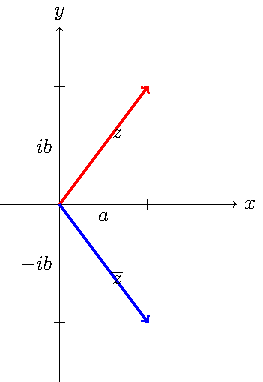
\includegraphics{complex_conjugate.pdf}
% \end{figure}

The complex conjugate of $z$ in this plane is described by a vector that is symmetric with respect to the real axis.

The sum of 2 complex numbers can be described as a sum of two vectors that start at the origin: the diagonal of the parallelogram that is constructed out of those 2 vectors.

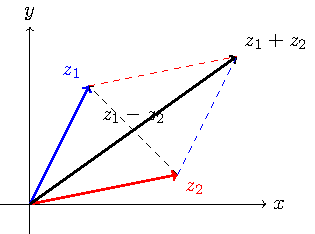
\includegraphics{sum_complex.pdf}

The difference between 2 complex numbers is the second(shorter) diagonal of the same parallelogram.
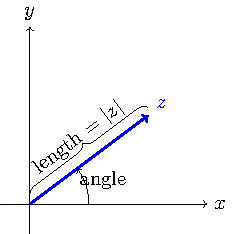
\includegraphics{length_angle_complex.pdf}

Recall: any vector is uniquely determined by its length and the angle that it creates with the $x$-axis [in the counterclockwise, positive direction]

\begin{definition}[Alternative]
 The distance from the origin $(0,0)$ to the point $z = (x,y)$ is called the modulus of the complex number $z$.
\end{definition}
Let us assume that this is the only definition and obtain previous definition from it.
By the Pythagorean theorem we get:
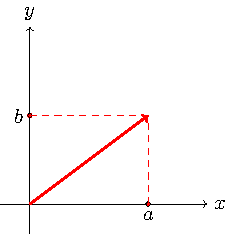
\includegraphics{coordinates_complex.pdf}

$\lvert z\rvert = \sqrt{a^2+b^2}(= \lvert a+ib \rvert)$. This is exactly the previous modulus definition.

\begin{example}
Compute $\lvert z\rvert$ for $z_1=7+9i$, $z_2=4-3i$.
$\lvert z_1\rvert = \lvert 7+9i\rvert = \sqrt{7^2+9^2} = \sqrt{130}$
$\lvert z_2\rvert = \lvert 4-3i\rvert = \sqrt{4^2+(-3)^2} = \sqrt{25} = 5$

Check (very easy!): The distance between any two points
$z=(x,y)$ and $z_0=(x_0,y_0)$ is
\[ \lvert z-z_0\rvert = \lvert (x-x_0)+i(y-y_0)\rvert = \sqrt{(x-x_0)^2+(y-y_0)^2} \]
\end{example}

The equations $\lvert z_1 \rvert =\sqrt{130}$, $\lvert z_2 \rvert =5$ describe the geometric place of all the points $z$ that are at distance $\sqrt{130}$ or $5$ from the origin - namely, it is a circle. In general we have:
Circle with radius $R$ centered at $z_0$: $\lvert z-z_0\rvert = R$.
\begin{example}
$\lvert z+1+i\rvert = 2$: circle centered at $z_0 = -(1+i)$ of radius $2$.

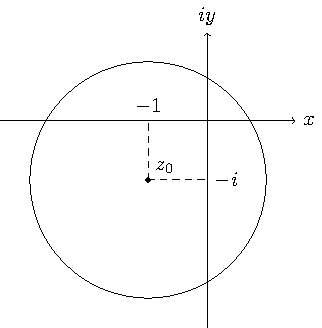
\includegraphics{circle_coord_cmplx.pdf}

Indeed, all the points for which this equation holds lie on the circle described by $\sqrt{(x+1)^2+(y+1)^2} = 2$
\end{example}

The equation $\lvert z-z_0 \rvert <R$ describes all the points that lie inside the circle centered at $z_0$ of radius $R$ (but not on the circle!). 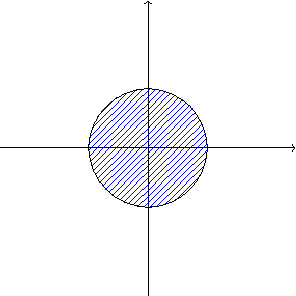
\includegraphics{filled_circle.pdf}

\begin{example}
 Find the geometric place of the points $z$ for which $\lvert z+2 \rvert - \lvert z-2\rvert = 1$
\end{example}
We are looking for the geometric place of all points $z$ such that the difference of distances from the point $z$ to two points $z=2$ and $z=-2$ is $1$. Let us show that this is a hyperbola.
Recall: hyperbola equation $\frac{x^2}{a^2} - \frac{y^2}{b^2} = 1$ - hyperbola with vertices at $(a,0)$ and $(-a,0)$ with asymptotes at $y=\pm \frac{b}{a}x$.

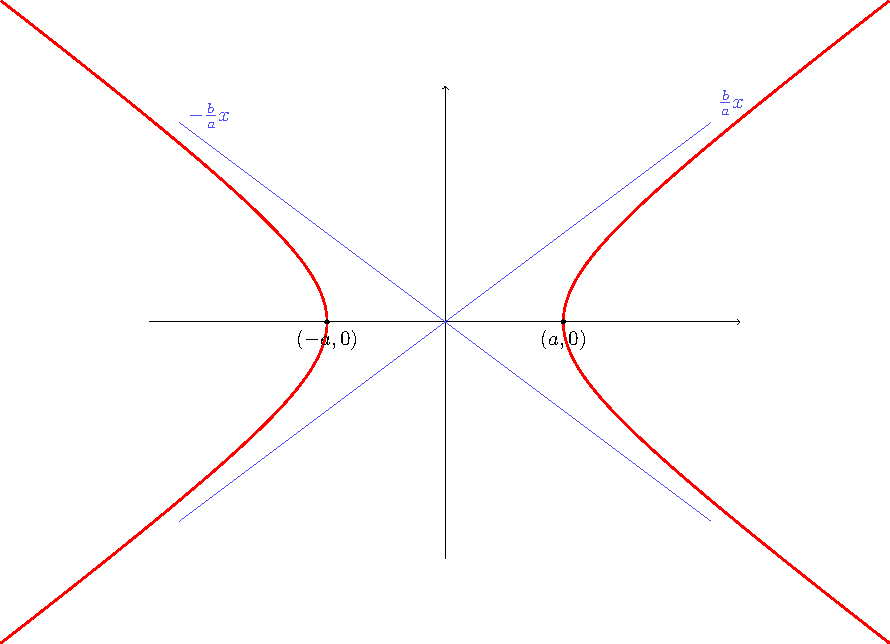
\includegraphics[width=0.7\textwidth]{hyperbola_cmplx.pdf}

For $-\frac{y^2}{b^2}+\frac{x^2}{a^2} = 1$: the vertices are at $(0,b)$ and $(0,-b)$ and asymptotes at $y=\pm \frac{b}{a}x$.

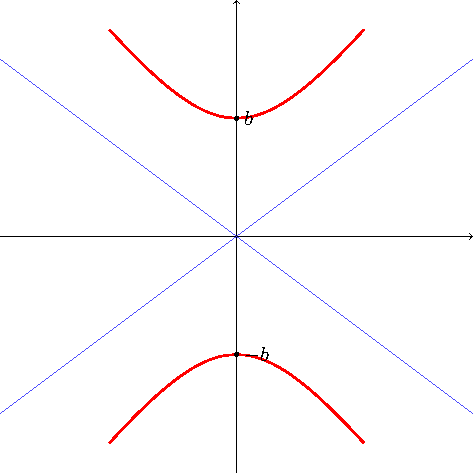
\includegraphics{hyperbola2-cmplx.pdf}

% 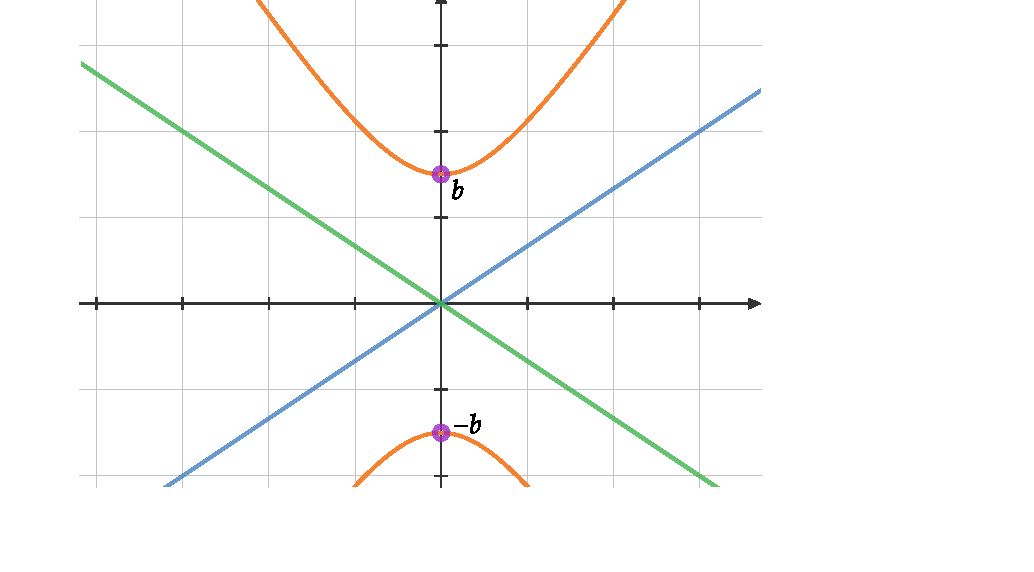
\includegraphics{hyperbola2-complex.pdf}
Here we have:
$ \lvert z+2 \rvert -\lvert z-2\rvert = 1 \implies \lvert x+iy+2\rvert - \lvert x+iy-2\rvert = 1 $
$ \implies \lvert (x+2)+iy\rvert-\lvert(x-2)+iy\rvert = 1 \implies \sqrt{(x+2)^2+y^2} - \sqrt{(x-2)^2+y^2} = 1 $
$ \implies \sqrt{(x+2)^2+y^2} = 1 + \sqrt{(x-2)^2+y^2} \iff (x+2)^2+y^2 = 1 + (x-2)^2+y^2 + 2\sqrt{(x-2)^2+y^2} $
$ \iff (x+2)^2 - (x-2)^2 -1 = 2\sqrt{(x-2)^2+y^2} \iff x^2+4x+4-x^2+4x-4-1 = 2\sqrt{(x-2)^2+y^2} $
$ \iff 8x-1 = 2\sqrt{(x-2)^2+y^2} \iff (8x-1)^2 = 4((x-2)^2+y^2) $
$ \iff 64x^2-16x+1 = 4x^2-16x+16+4y^2 \implies 60x^2-4y^2 = 15$
$ \iff 4x^2 - \frac{y^2}{15/4} = 1 \iff \frac{x^2}{1/4} - \frac{y^2}{15/4} = 1 \iff \frac{x^2}{(1/2)^2} - \frac{y^2}{(\sqrt{15}/2)^2} = 1 $
Thus, this is a hyperbola with vertices at $(\pm \frac{1}{2}, 0)$ with asymptotes $y= \pm\frac{\sqrt{15}/2}{1/2}x = \pm \sqrt{15}x$

Now we define the second object needed for a unique definition of a vector - an angle. This angle is called the argument of a complex number.

\begin{definition}
An \emph{argument} of $z \neq 0$, denoted by $\arg z$, is an angle $\theta$ such that $\cos\theta = \frac{\Re z}{\lvert z\rvert}$, $\sin \theta = \frac{\Im z}{\lvert z\rvert}$.
\end{definition}
 It is only defined up to the addition of multiples of $2\pi$. We say that $\theta$ is the \emph{principle value} of the argument if $0\leq \theta < 2\pi$ and denote the principal value of the argument $z$ by $\text{Arg} z$.

 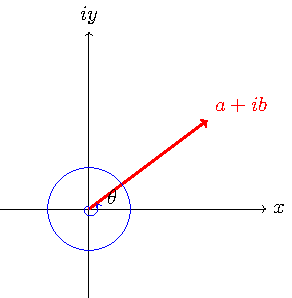
\includegraphics{angle_complex.pdf}
 
 The argument is exactly the angle that the vector $z$ creates with the $x$-axis when measured following the positive (anti-clockwise) direction.
 As we said: the argument takes infinitely many values that differ one from another by a multiple of $2\pi$.
 So, now we have 3 ways to represent a complex number: as an ordered pair, an algebraic form $x+iy$, or via its modulus and an argument.
 Representation: $z=(x,y), z=x+iy$, or $x= \lvert z\rvert\cos\theta, y=\lvert z\rvert\sin\theta \implies z=\lvert z\rvert(\cos\theta + i\sin\theta)$ Polar form ($r,\theta$ - coordinates.)
 The last form is called the polar form of a complex number.

It is more convenient to use the algebraic form to add complex numbers and it is easier to multiply using the polar form. Let us see how we pass from an algebraic to polar representation.

\begin{example}
 Write the following numbers in polar form:
 \begin{enumerate}[label=(\alph*)]
    \item $-2+2i$ 
    \item $2$ 
    \item $-i$
\end{enumerate}
    \begin{soln}
\begin{enumerate}[label=\alph*)]
    \item $z=-2+2i \implies \lvert z\rvert = \sqrt{(-2)^2+2^2} = 2\sqrt{2}$, $\cos\theta = \frac{-2}{2\sqrt{2}} = -\frac{1}{\sqrt{2}}$, $\sin\theta = \frac{2}{2\sqrt{2}} = \frac{1}{\sqrt{2}} \implies \theta = \frac{3\pi}{4}(+2\pi k, k\in \mathbb{Z}) \implies z = 2\sqrt{2}(\cos\frac{3\pi}{4}+i\sin\frac{3\pi}{4})$
    \item $z=2 \implies \lvert z\rvert = \sqrt{2^2+0^2} = 2$, $\cos \theta = \frac{2}{2} = 1$, $\sin\theta = \frac{0}{2} = 0 \implies \theta = 0(+2\pi k, k\in \mathbb{Z}), z=2(\cos 0 + i\sin 0)$
    \item $z=-i \implies \lvert z\rvert = \sqrt{0^2+(-1)^2} = 1$, $\cos\theta = \frac{0}{1} = 0$, $\sin\theta = \frac{-1}{1}=-1 \implies \theta = \frac{3\pi}{2}(+2\pi k, k\in \mathbb{Z}) \implies z = 1(\cos(\frac{3\pi}{2})+i\sin(\frac{3\pi}{2}))$
\end{enumerate}
    \end{soln}
\end{example}

 In all previous examples the argument is up to the addition of $2\pi k$.
 \begin{remark}
$a \equiv b(\text{mod } c)$: means that there exists an integer $k\in\mathbb{Z}$ s.t. $a-b=kc$.
In particular, if $c=2\pi$, then $a\equiv b(\text{mod } 2\pi)$ means that there exists $k \in \mathbb{Z}$ s.t. $a-b=2\pi k$.
\textbf{Important}: The argument of $z=0$ is not defined!
 \end{remark}
We have already studied some of the properties of the modulus in proposition~\ref{proposition:1.2}.

\begin{proposition}\label{proposition:1.2.5}
For any $z_1, z_2 \in \mathbb{C} (z_2\neq 0)$.
\begin{enumerate}
    \item $\lvert \bar{z}\rvert =\lvert z\rvert$
    \item $z\bar{z}=\lvert z\rvert^2$
    \item $\lvert \frac{z_1}{z_2} \rvert = \frac{ \lvert z_1 \rvert } { \lvert z_2 \rvert } $
\end{enumerate}
\end{proposition}
\begin{proof}    
    Here we present the proof of 1) via polar coordinates; 
    \verifythis the rest including the ones from proposition~\ref{proposition:1.2} (in the same way).
    Let $z = \lvert z\rvert(\cos\theta + i\sin\theta)$.
    $\bar{z} = \lvert z\rvert(\cos\theta - i\sin\theta)$
    $\lvert z\rvert = \lvert z\rvert\sqrt{\cos^2\theta + \sin^2\theta} = \lvert z\rvert$
    $\lvert \bar{z}\rvert = \lvert z\rvert\sqrt{\cos^2\theta + (-\sin\theta)^2} = \lvert z\rvert\sqrt{\cos^2\theta+\sin^2\theta} = \lvert z\rvert$
\end{proof}

Let us study the properties of the argument.
\begin{proposition}\label{proposition:1.3}
For any $z_1, z_2 \in \mathbb{C}(z_1, z_2 \neq 0)$
\begin{enumerate}
    \item $\arg(z_1z_2) = \arg z_1+\arg z_2$
    \item $\arg(\frac{z_1}{z_2}) = \arg z_1 - \arg z_2$
\end{enumerate}
\end{proposition}
Here we prove 1). Prove 2) in the same way.

\begin{proof}
Write $z_1,z_2$ in polar form: let $r_1 = \lvert z_1 \rvert $, $r_2 = \lvert z_2 \rvert $, $\phi_1 = \arg z_1$, $\phi_2 = \arg z_2$. Then $z_1 = r_1(\cos\phi_1+i\sin\phi_1)$ ,$z_2 = r_2(\cos\phi_2+i\sin\phi_2)$

$z_1/z_2 = r_1/r_2 (\cos\phi_1/\cos\phi_2 + i \sin\phi_1/\sin\phi_2)$
(4) $z_1z_2 = r_1r_2(\cos\phi_1\cos\phi_2 - \sin\phi_1\sin\phi_2+i(\sin\phi_1\cos\phi_2+\sin\phi_2\cos\phi_1)) = r_1r_2
= r_1r_2(\cos(\phi_1+\phi_2) + i\sin(\phi_1+\phi_2))$

Since $\arg z_1 = \phi_1 + 2\pi k$, $\arg z_2 = \phi_2 + 2\pi m \implies \arg(z_1z_2) = \phi_1 + \phi_2 + 2\pi n$, where $n = m + k$  (1)

\end{proof}

\begin{exercise}
    \begin{enumerate}
        \item $\implies$ The Geometric rule for multiplication: multiply moduli, add arguments.
        
        From rule: If $z_1 = z_2 = z$, from (4): $z^2 = r^2(\cos 2\phi + i\sin 2\phi)$.
        It is easy to prove by induction on $n$:
        \textbf{De Moivre formula} $z^n = \lvert z\rvert^n(\cos(n\phi) + i\sin(n\phi))$ \label{formula:De.Moivre}
    \end{enumerate}
\end{exercise}

\begin{example}
Express $\cos 3\alpha$ and $\sin 3\alpha$ in terms of $\cos\alpha$, $\sin\alpha$.

\begin{soln}  Construct complex number $z = \cos\alpha + i\sin\alpha$. By De Moivre formula $z^3 = \cos 3\alpha + i\sin 3\alpha$. On the other hand:
$z^3 = (\cos\alpha + i\sin\alpha)^3 = \cos^3\alpha + 3i\cos^2\alpha\sin\alpha + 3i^2\cos\alpha\sin^2\alpha + i^3\sin^3\alpha = \cos^3\alpha - 3\cos\alpha\sin^2\alpha + i(3\cos^2\alpha\sin\alpha - \sin^3\alpha)$

By the equality definition: $z_1=z_2 \iff \Re(z_1) = \Re(z_2)$ and $\Im(z_1) = \Im(z_2)$.
Let us compare these two expressions:
$\cos 3\alpha + i\sin 3\alpha = \cos^3\alpha - 3\cos\alpha\sin^2\alpha + i(3\cos^2\alpha\sin\alpha - \sin^3\alpha)$
$\implies \cos 3\alpha = \cos^3\alpha - 3\cos\alpha\sin^2\alpha$
$\sin 3\alpha = 3\cos^2\alpha\sin\alpha - \sin^3\alpha$
\end{soln}
\end{example}

\begin{example}
Define $\frac{1}{z}$ geometrically.

\begin{soln}  Let us compute the modulus and the argument.
By proposition~\ref{proposition:1.2.5} part 3): $\lvert \frac{1}{z}\rvert = \frac{1}{\lvert z\rvert}$ and since $z\cdot \frac{1}{z} = 1$
$0 = \arg 1 = \arg(z\cdot \frac{1}{z}) = \arg z + \arg \frac{1}{z} \implies \arg \frac{1}{z} = -\arg z$
\end{soln}
\end{example}

\subsection{Roots and Euler's formula}

\begin{definition}
$n$-th root of a complex number $z$ is a complex number $w$ such that $z = w^n$ (Notation: $\sqrt[n]{z} = w$)
\end{definition}

\begin{example}
Find the formula for computing roots of a given $z \in \mathbb{C}$.

\begin{soln}  Let $z=w^n$, let us write $z$ and $w$ in polar form.
$z = r(\cos\psi + i\sin\psi)$
$w = \rho(\cos\theta + i\sin\theta)$

Now we express $\rho$ and $\theta$ in terms of $r$ and $\psi$ ($r, \psi$ are given!).
From the definition: $z=w^n$ or $r(\cos\psi + i\sin\psi) = \rho^n(\cos(n\theta) + i\sin(n\theta))$
$\implies \rho^n = r$, $\cos(n\theta) = \cos\psi$, $\sin(n\theta) = \sin\psi \implies \rho = \sqrt[n]{r}$, $\theta = \frac{\psi + 2\pi k}{n}$ for $0\leq k \leq n-1$.
It is easy to see (check!) that for $k>n-1$ we will get again the same values!. Thus, we obtain
\begin{equation}\label{equation:244.1}
    w = \sqrt[n]{r}(\cos(\frac{\psi + 2\pi k}{n}) + i\sin(\frac{\psi + 2\pi k}{n})), \quad k=0,1,2,\ldots,n-1. \tag{**}
\end{equation}
\end{soln}
\end{example}

\begin{corollary}
$n$-th root of a complex number takes exactly $n$ different values that are placed on the vertices of a regular polygon with $n$ sides inscribed in a circle centered at 0 of radius $\sqrt[n]{\lvert z\rvert}$.
\end{corollary}

Recall: regular polygon is a polygon whose sides and angles are equal.

\begin{example}
Compute $\sqrt[4]{1-i}$.

\begin{soln}  We need to compute the modulus and the argument of 1-i.
$\lvert 1-i\rvert = \sqrt{1^2+(-1)^2} = \sqrt{2}$, $\cos\theta = \frac{1}{\sqrt{2}}$, $\sin\theta = \frac{-1}{\sqrt{2}} \implies \theta = \frac{7\pi}{4} + 2\pi k$ (or $\theta = -\frac{\pi}{4} + 2\pi k$)
$\implies 1-i = \sqrt{2}(\cos\frac{7\pi}{4} + i\sin\frac{7\pi}{4})$ - the polar form of 1-i.

Using formula (\ref{equation:244.1}) we get
$w = \sqrt[n]{1-i} = 2^{1/8}(\cos(\frac{7\pi/4 + 2\pi k}{4}) + i\sin(\frac{7\pi/4 + 2\pi k}{4}))$, $k=0,1,2,3$
$k=0: \quad 2^{1/8}(\cos\frac{7\pi}{16} + i\sin\frac{7\pi}{16}) \approx 0.21 + i1.07$
$k=1: \quad 2^{1/8}(\cos\frac{15\pi}{16} + i\sin\frac{15\pi}{16}) \approx -1.07 + i0.21$
$k=2: \quad 2^{1/8}(\cos\frac{23\pi}{16} + i\sin\frac{23\pi}{16}) \approx -0.21 - i1.07$
$k=3: \quad 2^{1/8}(\cos\frac{31\pi}{16} + i\sin\frac{31\pi}{16}) \approx 1.07 - i0.21$

Let us draw these roots on a circle, centered at $0$ of radius $2^{1/8}$. Connecting the neighboring roots we obtain a square.

\end{soln}
\end{example}

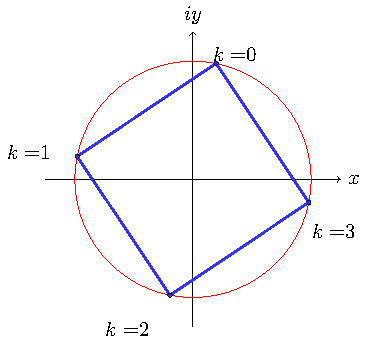
\includegraphics{circle_square.pdf}


\begin{example}
Compute all the roots of $z = \sqrt[4]{-4}$.

\begin{soln}  $\lvert -4\rvert = 4$, $\cos\theta = \frac{-4}{4} = -1$, $\sin\theta = \frac{0}{4} = 0 \implies \theta = \pi + 2\pi k$
From (\ref{equation:244.1}) we get
$\sqrt[4]{-4} = 4^{1/4}(\cos\frac{\pi + 2\pi k}{4} + i\sin\frac{\pi + 2\pi k}{4}) = \sqrt{2}(\cos(\frac{\pi}{4} + \frac{\pi k}{2}) + i\sin(\frac{\pi}{4} + \frac{\pi k}{2}))$ for $k=0,1,2,3$.
$k=0: \quad \sqrt{2}(\cos\frac{\pi}{4} + i\sin\frac{\pi}{4}) = \sqrt{2}(\frac{1}{\sqrt{2}} + i\frac{1}{\sqrt{2}}) = 1+i$
$k=1: \quad \sqrt{2}(\cos\frac{3\pi}{4} + i\sin\frac{3\pi}{4}) = \sqrt{2}(-\frac{1}{\sqrt{2}} + i\frac{1}{\sqrt{2}}) = -1+i$
$k=2: \quad \sqrt{2}(\cos\frac{5\pi}{4} + i\sin\frac{5\pi}{4}) = \sqrt{2}(-\frac{1}{\sqrt{2}} - i\frac{1}{\sqrt{2}}) = -1-i$
$k=3: \quad \sqrt{2}(\cos\frac{7\pi}{4} + i\sin\frac{7\pi}{4}) = \sqrt{2}(\frac{1}{\sqrt{2}} - i\frac{1}{\sqrt{2}}) = 1-i$

%\begin{wrapfigure}[]{r}{0.5\textwidth}
%    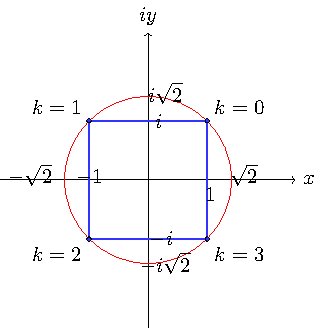
\includegraphics{circle_square2.pdf}
%\end{wrapfigure}

%\begin{figure}[htbp] % htbp = here, top, bottom, page (placement preference)
%    \centering
    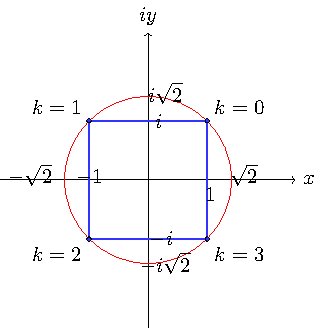
\includegraphics[width=0.5\textwidth]{circle_square2.pdf}
    % \caption{Optional: Roots of $z=\sqrt[4]{-4}$} % Add caption if needed
    % \label{fig:circle_square2} % Add label if needed
%\end{figure}
\end{soln}
\end{example}

The following formula is one of the most celebrated formulas in mathematics.

\begin{theorem}[Euler's formula; Euler 1760]\label{theorem:1.1}
Let $\theta \in \mathbb{R}$. Then $\cos\theta + i\sin\theta = e^{i\theta}$ where $e^{i\theta}$ denotes the sum of the power series $e^{i\theta} = 1 + i\theta + \frac{(i\theta)^2}{2!} + \frac{(i\theta)^3}{3!} + ... = \sum_{n=0}^{\infty}\frac{(i\theta)^n}{n!}$.
\end{theorem}

Set $\theta = \pi$. From this formula: $e^{i\pi} = -1$ - we have connected $-1$, $e$, $i$, $\pi$ in one formula!

We cannot prove this theorem now: first, we will need to examine the properties of the power series, however, we shall use it as a convenient notation even before we proved it. From the formula:
$\Re e^{i\theta} = 1 - \frac{\theta^2}{2!} + \frac{\theta^4}{4!} - ... = $ The Taylor series for $\cos\theta$ (about $\theta = 0$)
$\Im e^{i\theta} = \theta - \frac{\theta^3}{3!} + \frac{\theta^5}{5!} - ... = $ The Taylor series for $\sin\theta$ (about $\theta = 0$)

This formula provides a way of conversion between Cartesian coordinates $x+iy$ and the polar form (modulus and argument) as follows:
If $z\neq 0$: $\lvert z\rvert=r$, $\arg z = \theta \implies z = re^{i\theta}$ (the polar form)

Then $\bar{z} = x-iy = r(\cos\theta - i\sin\theta) = re^{-i\theta}$.
The following should be true:
$e^{i\theta} = e^{i(\theta + 2\pi n)}$ for every $n\in\mathbb{Z}$ (Euler's formula)
$e^{i(\phi + \psi)} = e^{i\phi}e^{i\psi}$
$\frac{1}{e^{i\theta}} = e^{-i\theta}$
$(e^{i\theta})^n = e^{in\theta}$ for every $n\in\mathbb{Z}$.

These facts are easily proved using theorem~\ref{theorem:1.1}, but they are not obvious, 
since $e^{i\theta}$ means $1 + i\theta + \frac{(i\theta)^2}{2!} + ...$ and raising the real 
number $e$ to the purely imaginary power $i\theta$ is not well-defined at the moment.